\chapter{Stos technologiczny}
\label{cha:stosTechnologiczny}

{\it

W celu realizacji wymagań stawianych opracowywanym aplikacjom wykorzystane zostały różne technologie umożliwiające implementację określonych aspektów dostarczanych funkcjonalności.

Wdrożenie zabezpieczeń dostępu do aplikacji oparte zostało na mechanizmach bezpieczeństwa definiowanych przez specyfikację Java EE i dostarczanych przez serwer aplikacyjny JBoss. Serwer JBoss pozwala konfigurować systemy i domeny bezpieczeństwa oraz stosowane w ich obrębie mechanizmy uwierzytelniania i autoryzacji użytkowników usług. Proces uwierzytelniania klientów aplikacji wykorzystuje mechanizmy implementowane poprzez protokół LDAP. 

Przykładowe aplikacje wykorzystują realizację standardu SAML - projekt Picketlink. Picketlink definiuje model tożsamości wykorzystywany w procesie uwierzytelniania, pozwala na stosowanie standardu - WS-Trust w celu obsługi funkcjonalności federacji tożsamości. Dostarcza implementację modułów ,,Identity Provider'' oraz ,,Security Token Service''. 

}

%---------------------------------------------------------------------------
\autsection{Mechanizmy bezpieczeństwa platformy Java SE}{Krzysztof Wilaszek}
\label{sec:javaSE}

	Architektura platformy Java zaprojektowana została z uwzględnieniem różnorodnych aspektów bezpieczeństwa aplikacji komputerowych. Najbardziej podstawowe mechanizmy bezpieczeństwa dotyczą poziomu języka programowania - można wśród nich wymienić bezpieczeństwo typów, automatyczne zarządzanie pamięcią, mechanizm \textit{,,garbage collection''} czy też mechanizm bezpiecznego ładowania klas. Składnia języka Java umożliwia również definiowanie modyfikatorów dostępu do pól i metod klas. Kod napisany w języku Java kompilowany jest do niezależnego od platformy kodu bajtowego, który przed wykonaniem weryfikowany jest pod kątem składni, zarządzania pamięcią, operacji na stosie czy też bezpieczeństwa typów\cite{Oracle13}.

	Wraz z rozwojem platformy Java wprowadzano zmiany w architekturze bezpieczeństwa Javy wzbogacając funkcjonalności platformy o powszechnie wykorzystywane algorytmy, mechanizmy i protokoły. Należą do nich algorytmy kryptograficzne, interfejsy dla infrastruktury klucza publicznego, interfejsy uwierzytelniania i kontroli dostępu do zasobów aplikacji. Platforma Javy zapewnia niezależność aplikacji wykorzystujących API mechanizmów bezpieczeństwa od konkretnej, niejednokrotnie złożonej implementacji danego mechanizmu. Umożliwia również dostarczenie własnej realizacji dla różnych mechanizmów bezpieczeństwa.

	\subsection{Architektura platformy Java SE dla mechanizmów bezpieczeństwa}

		Podstawowymi założeniami architektury platformy Javy dla mechanizmów bezpieczeństwa są niezależność aplikacji wykorzystującej konkretne mechanizmy bezpieczeństwa od ich implementacji, zdolność do współpracy pomiędzy różnymi aplikacjami i serwisami bezpieczeństwa oraz rozszerzalność zbioru dostarczanych mechanizmów bezpieczeństwa. Podstawowym elementem architektury bezpieczeństwa platformy Java realizującym te założenia jest klasa \textit{java.security.Provider}. Klasa dostarcza implementacji określonych usług bezpieczeństwa. Dostawcom usług bezpieczeństwa przyporządkowane mogą być priorytety - w przypadku kilku implementacji tego samego serwisu wybierany jest ten od dostawcy z najwyższym priorytetem. 

		Implementacja platformy Java zawiera zbiór gotowych dostawców dla różnych usług bezpieczeństwa takich jak kryptografia, uwierzytelnianie, etc. Zgodnie z założeniami architektonicznymi zbiór funkcjonalności może być rozszerzany oraz wykorzystywany przez różnorodne współpracujące aplikacje. Usługi mogą być konfigurowane w celu ich dostosowania do potrzeb konkretnych aplikacji. 

	\subsection{Usługi bezpieczeństwa platformy Java SE}

		Platforma Java udostępnia szeroki wachlarz usług dostarczających funkcjonalności algorytmów kryptograficznych takich jak MDA, podpis cyfrowy, szyfrowanie symetryczne(blokowe i strumieniowe) oraz asymetryczne, szyfrowanie przy użyciu haseł, kryptografia krzywych eliptycznych, protokół uzgadniania kluczy, generator kluczy, kod uwierzytelniania wiadomości, generator liczb pseudolosowych. Dostarcza implementacji bezpiecznej wymiany wiadomości przy użyciu infrastruktury klucza publicznego(ang. \textit{Public Key Infrastructure}). Jest to podejście, w którym tożsamość klientów aplikacji potwierdzana jest przez certyfikaty cyfrowe generowane przez \textit{Certification Authorities}. Platforma Javy dostarcza implementacji wspierających certyfikaty X.509 oraz listy unieważnionych certyfikatów(ang. \textit{Certificate Revocation Lists}). Platforma dostarcza mechanizmów przechowywania kluczy i certyfikatów bezpieczeństwa w oparciu o różne standardy. Dostarcza API i narzędzi umożliwiających operacje na zgromadzonych danych.

		Platforma Javy dostarcza również API umożliwiające uwierzytelnianie klientów aplikacji przy użyciu modułów logowania. Architektura podsystemu uwierzytelniania umożliwia wprowadzanie nowych modułów logowania rozszerzających dostępne funkcjonalności uwierzytelniania. Domyślnie dostępne są metody uwierzytelniania oparte o protokoły LDAP i Kerberos oraz o dane zgromadzone w magazynach kluczy.

		W ramach platformy Java zaimplementowane zostały mechanizmy zapewnienia bezpieczeństwa komunikacji sieciowej - gwarantowania poufności komunikacji oraz zapewnienia integralności danych. Jednym z tych mechanizmów są protokoły SSL oraz TLS dostarczające funkcjonalności  szyfrowania przesyłanych danych, weryfikacji ich integralności oraz uwierzytelniania klienta i serwera. Platforma dostarcza również implementacji standardu SASL opisującego proces uwierzytelniania w komunikacji między klientem i serwerem. 

		Innym ważnym mechanizmem implementowanym w ramach usług bezpieczeństwa platformy Java jest mechanizm kontroli dostępu do zasobów aplikacji. Moduł kontroli dostępu oparty jest o managera bezpieczeństwa(ang. \textit{security manager})  podejmującego decyzję o przydzieleniu lub odmowie dostępu do określonych zasobów aplikacji. Decyzja ta podejmowana jest na podstawie informacji skojarzonych z kodem aplikacji na etapie jego ładowania przez \textit{class loadera}  takich jaki pochodzenie kodu, jednostka podpisująca kod oraz uprawnienia przyznane kodowi. W procesie podejmowania decyzji uwzględniane są polityki zdefiniowane w obrębie aplikacji. 

		Platforma dostarcza również implementacji standardu cyfrowego podpisu XML gwarantującego integralność danych oraz uwierzytelnienie wiadomości i jej nadawcy.
	
%---------------------------------------------------------------------------

\autsection{Mechanizmy bezpieczeństwa platformy Java EE}{Krzysztof Wilaszek}
\label{sec:javaEE}

	Specyfikacja Java EE definiuje mechanizmy bezpieczeństwa dla komponentów wchodzących w skład poszczególnych warstw aplikacji. Implementacja mechanizmów bezpieczeństwa dla komponentów dostarczana jest przez kontener aplikacji. Istnieją dwa rodzaje definiowania wymagań bezpieczeństwa aplikacji - deklarowalne i programowalne\cite{Oracle12}. Deklarowalna definicja bezpieczeństwa aplikacji jest to opis wymagań bezpieczeństwa zapisany przy użyciu adnotacji lub deskryptora aplikacji. Przy użyciu tej metody możliwe jest zdefiniowanie ról, ograniczeń dostępu do poszczególnych zasobów aplikacji oraz wymagań dotyczących procesu uwierzytelniania użytkowników. Drugie podejście - programowalna definicja bezpieczeństwa aplikacji jest opisem wymagań bezpieczeństwa zawartym w kodzie aplikacji, służącym podejmowaniu decyzji dotyczących bezpieczeństwa aplikacji na etapie realizacji jej funkcjonalności. Podejście to jest najczęściej wykorzystywane gdy metoda oparta o deklaracje jest niewystarczająca w danej sytuacji.

	Na aplikację Java EE mogą składać się zasoby chronione i niechronione. Kontrola dostępu do zasobów chronionych możliwa jest dzięki procesowi autoryzacji. Proces autoryzacji oparty jest o identyfikację tożsamości klienta aplikacji oraz uwierzytelnienie zidentyfikowanej tożsamości klienta. Rozwiązania dostarczane przez platformę Java EE skupiają się na aspektach bezpieczeństwa związanych z uwierzytelnianiem, autoryzacją dostępu do zasobów aplikacji, zapewnianiem integralności danych oraz poufności przekazywania informacji, logowaniem transakcji, audytami i zagadnieniami zapewniania jakości dostarczanych usług(ang. \textit{Quality of Service}). Mechanizmy bezpieczeństwa platformy Java EE dostarczane są przez kontener komponentów aplikacji. 

	\subsection{Poziomy mechanizmów bezpieczeństwa platformy Java EE}

		Mechanizmy bezpieczeństwa platformy Java EE dostarczane są na różnych poziomach - na poziomie warstwy aplikacji, warstwy transportowej lub na poziomie wiadomości.

		Mechanizmy bezpieczeństwa na poziomie aplikacji to usługi bezpieczeństwa dostarczane przez kontener aplikacji do wykorzystania przez konkretne aplikacje. Mechanizmy tego typu charakteryzują się łatwością konfiguracji i implementacji oraz pozwalają na dokładne dopasowanie pomiędzy mechanizmami kontroli dostępu do aplikacji a aplikacjami. Wadą rozwiązań tego typu jest brak możliwości zapewnienia bezpieczeństwa zasobów aplikacji poza jej środowiskiem. Ma to szczególnie duże znaczenie dla aplikacji i usług sieciowych. Dlatego mechanizmy bezpieczeństwa warstwy aplikacji powinny być uzupełnione mechanizmami warstwy transportowej i mechanizmami na poziomie przesyłanych wiadomości. 

		Zabezpieczenia warstwy transportowej dostarczane są przez mechanizmy przesyłania wiadomości pomiędzy dostawcami a klientami usług. Mechanizmy bezpieczeństwa warstwy transportowej platformy Java EE oparte są o szyfrowaną wersję protokołu HTTP - HTTPS wykorzystująca protokół SSL(\textit{Secure Sockets Layer}). Są to mechanizmy stosowane w połączeniach punkt - punkt pomiędzy nadawcą a odbiorcą. Umożliwiają uwierzytelnianie klienta i serwera, pozwalają gwarantować integralność i poufność przesyłanych informacji. Zawierają mechanizmy negocjacji algorytmów szyfrowania i kluczy kryptograficznych. Mechanizmy bezpieczeństwa warstwy transportowej gwarantują ochronę wiadomości na drodze pomiędzy nadawcą a odbiorcą. Rozwiązania oparte o protokół SSL wykorzystują certyfikaty cyfrowe w procesie uwierzytelniania uczestników komunikacji. 

		Zastosowanie mechanizmów bezpieczeństwa poziomu wiadomości polega na dołączeniu informacji bezpieczeństwa do przesyłanych wiadomości lub ich załączników. Informacja bezpieczeństwa może dotyczyć całości informacji lub jej części i jest z nią związana na całej drodze pomiędzy nadawcą a odbiorcą. Zastosowanie mechanizmów tego typu pozwala na bezpieczne przesyłanie informacji pomiędzy nadawcą a odbiorcą z pośrednictwem dowolnych węzłów komunikacyjnych. Ma na celu zagwarantowanie, że tylko odbiorca będzie w stanie odczytać zabezpieczone informacje.

	\subsection{Zastosowanie domen bezpieczeństwa w aplikacjach platformy Java EE}

		Mechanizmy bezpieczeństwa platformy Java EE oparte są o koncepcję domen bezpieczeństwa. W ramach domen bezpieczeństwa istnieją użytkownicy przypisani do różnych ról oraz klasyfikowani w ramach grup. Zastosowanie ról pozwala na przyznanie dowolnym klientom uprawnień do określonych zasobów aplikacji. Dzięki użyciu grup możliwe jest zbiorcze określenie uprawnień użytkowników przypisanych do grup. Określenie uprawnień do zasobów aplikacji możliwe jest między innymi dzięki użyciu adnotacji - \textit{@RolesAllowed}, \textit{@PermitAll}, \textit{@DenyAll}.
		
		\lstset{language=Java}
		\begin{lstlisting}
@RolesAllowed("RoleA")
public void forRoleA() {
	// Metoda dostępna dla użytkowników przypisanych do roli RoleA
}

@PermitAll
public void forAll(){
	// Metoda dostępna dla wszystkich użytkowników
}

@DenyAll
public void forbidden() {
	// Metoda niedostępna dla wszystkich użytkowników
}
		\end{lstlisting}		

%---------------------------------------------------------------------------

\autsection{Protokół LDAP}{Krzysztof Wilaszek}
\label{sec:ldap}

	LDAP(Lightweight Directory Access Protocol) jest protokołem definiującym metody, dzięki którym możliwy jest dostęp do danych zawartych w katalogach\cite{ZyTrax13}. Opisuje sposób reprezentacji danych w usłudze katalogowej oraz definiuje metody ładowania i eksportowania danych. Bazuje na standardzie X.500.

	\subsection{Model działania protokołu LDAP}

		\begin{figure}[h]
			\centering
			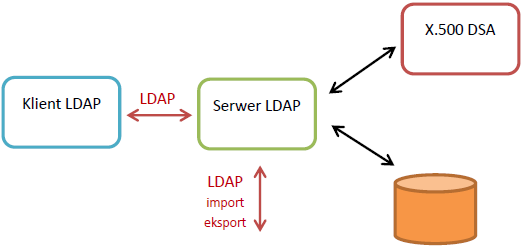
\includegraphics{img/ldap.png}
			\caption{Schemat funkcjonowania protokołu  LDAP}
			\label{Schemat funkcjonowania protokolu  LDAP}
		\end{figure}

		Protokół LDAP definiuje sposób dostępu do zasobów, nie określa natomiast sposób przechowywania danych. Jednym z wariantów jest przechowywanie informacji w bazie danych. Użytkownik komunikujący się z serwerem LDAP nie wie skąd pochodzą dane, które otrzymuje. Protokół LDAP definiuje również metody ładowania danych do usługi katalogowej oraz eksportowania danych z usługi przy użyciu formatu LDIF. Protokół LDAP opisuje operacje jakie mogą być wykonywane na modelu danych(np. modyfikowanie, usuwanie, odczyt).

	\subsection{Reprezentacja danych w protokole LDAP}

		Dane w protokole LDAP reprezentowane są w postaci hierarchii obiektów\cite{ZyTrax13}. Obiekty tworzą strukturę drzewa nazywanego drzewem DIT(Data Information Tree). Wierzchołek drzewa to element ,,root''. Każdy element drzewa składa się z co najmniej jednej klasy obiektów. Klasa obiektów to zbiór atrybutów przypisanych do obiektu. Każdy atrybut posiada nazwę i najczęściej ma przypisaną wartość. Klasa obiektu określa czy nadanie wartości danego atrybutu jest obowiązkowe czy opcjonalne. Obiekty identyfikowane są poprzez swoje położenie w drzewie - ścieżkę określającą elementy drzewa na drodze do obiektu. Identyfikator obiektu nazywany jest elementem Distinguished Name(DN).

	\subsection{Uwierzytelnianie przy użyciu protokołu LDAP}

		Usługa katalogowa LDAP może być wykorzystywana jako baza informacji o użytkownikach i serwis uwierzytelniający. LDAP pozwala również na przechowywanie informacji o rolach użytkowników. 

		Proces uwierzytelniania przy użyciu protokołu LDAP rozpoczyna się od pozyskania mapowania pomiędzy identyfikatorem użytkownika w systemie a elementem DN usługi katalogowej. Następnie wykonywana jest operacja uwierzytelniania w serwerze LDAP - ,,bind''. Aby wykonać operację ,,bind'' konieczne jest przesłanie nazwy DN i hasła użytkownika.  Innym sposobem uwierzytelnienia użytkownika może być porównanie przedstawionego przez niego hasła z hasłem przechowywanym przez usługę katalogową. Dla uwierzytelnionego użytkownika możliwe jest pobranie listy jego ról i uprawnień.

%---------------------------------------------------------------------------

\autsection{Mechanizmy bezpieczeństwa serwera aplikacyjnego JBoss}{Krzysztof Wilaszek}
\label{sec:jboss}

	Mechanizmy bezpieczeństwa serwera aplikacyjnego JBoss w wersji 7 oparte są o framework PicketBox. PicketBox dostarcza podstawowych funkcjonalności zapewnienia bezpieczeństwa dostępu do zasobów, takich jak uwierzytelnianie, autoryzacja, audyty systemu oraz mapowanie ról i danych uwierzytelniających. 

	\subsection{Podsystemy bezpieczeństwa serwera aplikacyjnego JBoss}

		Usługi bezpieczeństwa dostarczane przez Picketbox są dostępne dla serwera aplikacyjnego poprzez podsystem bezpieczeństwa(ang. Security Subsystem). Każdemu żądaniu klienta przypisywany jest kontekst bezpieczeństwa dostępny dla podsystemu bezpieczeństwa\cite{Lofthouse12}. 

		Kontekst bezpieczeństwa udostępnia komponenty skonfigurowane dla domeny bezpieczeństwa. Możliwe komponenty to:

		\begin{itemize}
			\item Authentication Manager - dokonuje uwierzytelniania użytkowników na podstawie otrzymanych danych uwierzytelniających przy użyciu modułów logowania zdefiniowanych dla wykorzystywanej domeny bezpieczeństwa;
			\item Authorization Manager - dostarcza informacji o rolach przypisanych użytkownikowi oraz dokonuje autoryzacji dostępu do zasobów dla uwierzytelnionych użytkowników;
			\item Audit Manager - pozwala na logowanie zdarzeń zachodzących w systemie zapewnienia bezpieczeństwa dostępu do aplikacji;
			\item Mapping Manager - pozwala na przypisywanie uwierzytelnionemu użytkownikowi dodatkowych uprawnień, ról lub atrybutów.
		\end{itemize}

		Korzystania z podsystemów bezpieczeństwa możliwe jest dzięki dodaniu rozszerzenia:
		\lstset{language=XML}
		\begin{lstlisting}
	<extension module="org.jboss.as.security"/>
		\end{lstlisting}
		w pliku konfiguracyjnym serwera.

		Podsystem bezpieczeństwa serwera aplikacyjnego JBoss udostępnia konfigurację następujących własności:

		\begin{itemize}
			\item security-management - pozwala nadpisywać domyślne parametry modułu PicketBox takie jak implementacje klas zarządców dla procesów uwierzytelniania, autoryzacji, audytów, mapowania danych tożsamości oraz tworzenia relacji zaufania.
			\item security-domains - pozwala na konfigurację domen bezpieczeństwa
			\item security-properties - pozwala definiować dodatkowe własności wymagane przez podsystem bezpieczeństwa.
		\end{itemize}

	\subsection{Domena bezpieczeństwa serwera aplikacyjnego JBoss}

		W ramach podsystemu bezpieczeństwa możliwa jest definicja domen bezpieczeństwa. Domena bezpieczeństwa opisuje mechanizmy zabezpieczeń dostępu do aplikacji wykorzystywane przez grupę usług przypisanych do tej domeny.

		Podstawowym zadaniem domeny bezpieczeństwa jest przeprowadzanie procesu uwierzytelniania klientów aplikacji. W tym celu do domeny przypisane są moduły logowania(ang. ,,Login Module'') wykorzystywane do uwierzytelniania użytkowników. Konfigurując moduł logowania należy wybrać klasę definiującą sposób i przebieg uwierzytelniania użytkownika. Domyślnie dostępne są implementacje pozwalające na uwierzytelnianie np. w oparciu o certyfikaty, bazę danych z użytkownikami i hasłami, protokół LDAP, protokół Kerberos lub prosty plik z użytkownikami i hasłami.

		Możliwe jest również oparcie mechanizmów uwierzytelniania o specyfikację JASPI(Java Authentication Service Provider Interface for Containers). JASPI definiuje standardowy interfejs dla dostawców usług, przy pomocy którego dla kontenera aplikacji Java EE możliwe jest uwierzytelnianie na podstawie danych bezpieczeństwa przesyłanych na poziomie wiadomości. Specyfikacja określa mechanizmy strony klienckiej oraz serwerowej. Serwer ma możliwość weryfikacji tokenów bezpieczeństwa lub podpisów przychodzących wiadomości i pozyskania opisu uprawnień użytkownika lub asercji. Strona kliencka może dodawać do wysyłanych wiadomości token bezpieczeństwa lub podpis cyfrowy. 

		Inny ważnym mechanizmem definiowanym na poziomie domeny bezpieczeństwa jest autoryzacja klientów aplikacji. Domyślnie realizowanym podejściem w procesie autoryzacji jest RBAC(Role Based Access Control). Metoda ta przydziela lub odmawia prawa dostępu do zasobów w oparciu o przynależność użytkownika do określonej grupy. Możliwe jest również użycie innych metod autoryzacji, np. JACC(Java Authorization Contract for Containers) lub XACML (eXtensible Access Control Markup Language). 

		Definicja domeny bezpieczeństwa obejmuje również:

		\begin{itemize}
			\item mapowania ról, uprawnień, danych uwierzytelniających i atrybutów; 
			\item konfigurację mechanizmu audytów operacji w domenie bezpieczeństwa
			\item konfigurację repozytorium certyfikatów bezpieczeństwa wykorzystywanych przez kontekst SSL lub przez procesy pozyskiwania i magazynowania certyfikatów.
		\end{itemize}

%---------------------------------------------------------------------------

\autsection{Picketlink}{Krzysztof Wilaszek}
\label{sec:picketlink}

Picketlink jest projektem dostarczającym implementacji założeń systemów zarządzania tożsamościami dla aplikacji Java. Picketlink definiuje model tożsamości wykorzystywanych w operacjach systemów IdM. Pozwala na zarządzanie informacjami o użytkownikach, grupach i rolach oraz ich atrybutach. Umożliwia wykorzystanie różnych sposobów przechowywania tożsamości, np. bazy danych lub usługi katalogowej LDAP. Projekt Picketlink umożliwia korzystanie z federacji tożsamości - wspiera specyfikacje SAML, OpenID oraz WS-Trust\cite{PicketLink13}.

Picketlink dostarcza wsparcie dla profili specyfikacji SAML umożliwiających jednokrotne uwierzytelnianie aplikacji webowych oraz globalne wylogowanie. Określa również mapowania dla protokołu HTTP przy użyciu komunikatów POST i Redirect. 

Picketlink implementuje mechanizmy pozwalające na tworzenie usługi ,,Identity Provider''. Dostarcza narzędzi konfiguracji usługi, uwierzytelniania a także implementację operacji obsługi przechowywania tożsamości. W ramach konfiguracji możliwe jest między innymi określenie zaufanych hostów dla usługi IdP, ustawienie cyfrowego podpisu dla wiadomości oraz szyfrowanie komunikatów. Usługa ,,Identity Provider'' w procesie uwierzytelniania może korzystać z mechanizmu domen bezpieczeństwa serwera aplikacyjnego JBoss. Dostawcy usług korzystają z serwisu IdP pozyskując asercje opisujące użytkowników. Picketlink umożliwia taką konfigurację usług aby ich mechanizmy uwierzytelniania korzystały z usługi IdP.

Narzędzia Picketlink dostarczają implementacji specyfikacji WS-Trust - za operacje zarządzania asercjami SAML(tworzenie, odnawianie, anulowanie i walidację) odpowiada usługa ,,Security Token Service''. Moduł Picketlink zawiera implementację usługi STS oraz pozwala konfigurować parametry takie jak szyfrowanie tokenu bezpieczeństwa i wymóg dołączania cyfrowego podpisu dla tokenów. Moduł implementuje narzędzia przechwytywania wywołań usług webowych i weryfikacji wymaganych asercji uprawniających do dostępu do zasobów. 

%---------------------------------------------------------------------------

\autsection{jBPM}{Tomasz Wójcik}
\label{sec:bpm}

jBPM jest narzędziem służącym do zarządzania procesami biznesowymi(Business Process Management). Pozwala ono na modelowanie, wykonywanie i monitorowanie procesów biznesowych. jBPM koncentruje się na wykonywalnych procesach biznesowych, a więc procesach napisanych w formalnych językach, które mogą być uruchomione przy pomocy silnika BPM.
Główną częścią jBPM jest silnik procesów biznesowych pozwalający na uruchomienie procesu zgodnego z językiem BPMN 2.0. Proces może być uruchomiony z poziomu języka Java, w dowolnym środowisku obsługującym tę platformę, także np. wewnątrz usługi w aplikacji typu SOA. 

Oprócz tego jBPM oferuje szereg innych komponentów w celu wspierania całego cyklu życia procesów biznesowych. Niektóre procesy biznesowe mogą zawierać zadania, które muszą zostać wykonane przez człowieka, np. potwierdzenie decyzji o przyznaniu kredytu lub uzyskanie podpisu klienta. jBPM oferuje wsparcie dla tego typu zadań, m.in. przy pomocy standardu WS-HumanTask. Framework pozwala na zdefiniowanie typu zadania, aktorów i danych związanych z zadaniem. Udostępnia również API, które może służyć do budowy aplikacji pośredniczącej w interakcji pomiędzy użytkownikami(aktorami) a systemem. API umożliwia np.  uzyskanie listy zadań zleconych danemu użytkownikowi, przypisanie zadania do innego użytkownika czy zmianę stanu zadania.
Niezawodność wykonywania procesów biznesowych jest krytyczna z punktu widzenia organizacji. Każdy rozpoczęty proces musi zostać zakończony, nawet w przypadku awarii systemu. Wykonanie niektórych złożonych procesów, szczególnie tych wykorzystujących aktorów ludzkich,  może zabierać długi okres czasu, liczony nawet w dniach. Co za tym idzie, bardzo ważną rzeczą jest zapewnienie persystencji i transakcyjności procesów. jBPM pozwala na zautomatyzowany zapis bieżącego stanu procesu w bazie danych. Gwarantuje także transakcyjność przy użyciu JTA lub systemu transakcji frameworku Spring.

Środowisko jBPM oferuje dwa zestawy narzędzi: workbench sieciowy, pozwalający na modelowanie, wykonywanie, zarządzanie i raportowanie procesów biznesowych oraz plug-in do środowiska Eclipse ułatwiający modelowanie, tworzenie, testowanie i debugowanie procesów.
jBPM udostępnia także API które służy do udostępniania procesu jako usługi, przy użyciu REST, RMI lub JMS. Integruje się z biblioteką Drools, dzięki której można definiować złożone reguły biznesowe i umieszczać je w ramach procesów.


%---------------------------------------------------------------------------

\autsection{SwitchYard}{Tomasz Wójcik}
\label{sec:switchyard}

SwitchYard jest lekkim frameworkiem wspierającym tworzenie, wdrażanie i zarządzanie aplikacjami zrealizowanymi zgodnie z paradygmatem SOA. Framework ten oferuje większość funkcji przypisywanych typowym rozwiązaniom typu Enterprise Service Bus i jest przez samych twórców określany jako, bardziej zorientowany na obsługę całego cyklu życia serwisów, następca projektu JBoss ESB. Dostarcza on środowiska uruchomieniowego pozwalającego na łatwą integrację różnorodnych komponentów systemu i udostępnienie ich w postaci wymaganej przez klienta.

SwitchYard wspiera strukturyzację systemu poprzez oddzielenie komponentów odpowiedzialnych za  przekształcanie i walidację wiadomości oraz tzw. cross-cutting concerns(np. transakcyjność) od kodu realizującego logikę biznesową. Framework udostępnia możliwość deklaratywnej transformacji wiadomości pomiędzy formatami JSON, XML(z wykorzystaniem JAXB lub transformat XSLT) i obiektami Javy lub dowolnym innym formatem dzięki użyciu konwerterów użytkownika. Umożliwia również walidację wiadomości z XML Schema lub przy użyciu własnych walidatorów. Framework pozwala też deklarować polityki np. dotyczące transakcyjności i bezpieczeństwa. Dzięki temu wiadomości które nie spełniają podanych kryteriów, przykładowo nie zawierają kontekstu transakcji, są automatycznie odrzucane. 

Każda aplikacja wykorzystująca framework SwitchYard zawiera deskryptor napisany w języku XML, zgodny ze standardem SCA (Service Component Architecture). Deskryptor ten opisuje ogólną strukturę aplikacji z podziałem na usługi, z wyszczególnieniem usług udostępnianych przez aplikację oraz zewnętrznych usług wykorzystywanych przez aplikację. 
Całość aplikacji zawarta jest w elemencie o nazwie kompozyt, który tworzy również nową przestrzeń nazw dla danej aplikacji. 
Podstawowym elementem warstwy wnętrza aplikacji jest komponent. Reprezentuje on fragment logiki aplikacji, dostarczany przez osobny element - implementację. Komponent może zostać zaimplementowany przy pomocy ścieżki przetwarzania z frameworku Apache Camel, procesu biznesowego z wykorzystaniem jBPM, zestawu reguł Drools lub klasy Javy. Komponent może dostarczać pewnej usługi(element component service) zdefiniowanej poprzez interfejs. Interfejs ten musi być zaimplementowany przez dany komponent. Komponent może także zdefiniować referencje do innych usług(component reference), które są wykorzystywane w jego implementacji. Mogą być to zarówno usługi lokalne jak i zewnętrzne.
Usługa kompozytu opisuje serwis dostępny z zewnątrz aplikacji, spełniający dany interfejs realizowany przez komponent zawarty w aplikacji. Usługa deklaruje sposób komunikacji z klientami zewnętrznymi poprzez element dowiązania usługi (service binding). 
Analogicznie, warstwa usług wymaganych przez aplikację składa się z referencji kompozytu, połączonych z referencjami komponentów, oraz dowiązań referencji, definiujących mechanizm komunikacji z usługami zewnętrznymi.
Łączenie ze sobą poszczególnych elementów systemu jest ułatwione dzięki zastosowaniu wzorca wstrzykiwania zależności, zgodnym ze standardem CDI(Contexts and Dependency Injection for Java EE).
SwitchYard udostępnia zestaw narzędzi do środowiska Eclipse, pozwalających na wizualizację struktury aplikacji. Poniższa grafika przedstawia opis poszczególnych elementów deskryptora aplikacji.

		\begin{figure}[h]
			\centering
			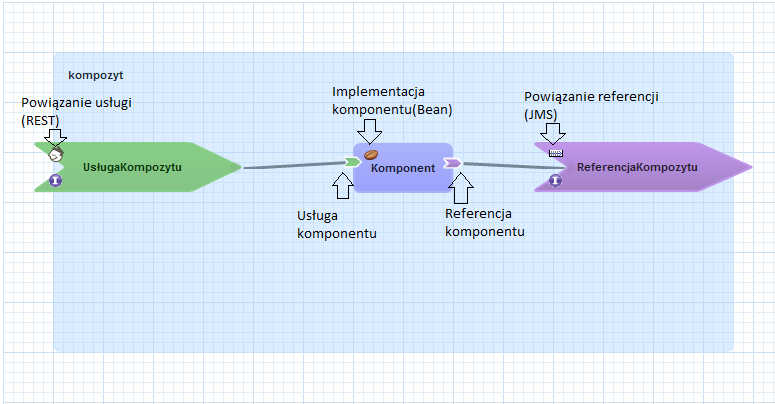
\includegraphics[width=\textwidth]{img/switchyard2.png}
			\caption{Elementy deskryptora aplikacji SwitchYard}
			\label{Elementy deskryptora aplikacji SwitchYard}
		\end{figure}

%---------------------------------------------------------------------------

\autsection{OpenShift}{Tomasz Wójcik}
\label{sec:openShift}

OpenShift jest środowiskiem typu Platform as a Service rozwijanym przez firmę Red Hat. Tworząc warstwę abstrakcji nad infrastrukturą z wykorzystaniem oprogramowania typu middleware i udostępniając zestaw odpowiednich narzędzi, platforma ta ułatwia tworzenie, wdrażanie i zarządzanie aplikacjami w wielu językach programowania. 

Środowisko OpenShift jest dostępne dla użytkowników w co najmniej dwóch postaciach. OpenShift Online to komercyjna usługa sieciowa, udostępniająca tworzenie aplikacji w chmurze publicznej. OpenShift Origin to otwarta wersja środowiska, która może być uruchomiona w dowolnej lokacji i w całości zarządzana przez użytkownika.
OpenShift jest zbudowany w oparciu o system Red Hat Enterprise Linux i może zostać uruchomiony wszędzie tam gdzie system ten działa, a więc także na np. maszynach wirtualnych. Architektura środowiska wyróżnia dwa rodzaje instancji systemu RHEL - node służy do uruchamiania aplikacji użytkowników, zaś broker ma za zadanie zarządzanie i orkiestrację instancji typu node. W ramach pojedynczej instancji node jest dostępnych wiele komponentów gear, które stanowią środowisko użytkownika końcowego, z zasobami ograniczonymi przy użyciu mechanizmów jądra systemu - Control Groups. Poszczególne komponenty gear są izolowane od siebie(multi-tenancy) za pomocą modułu SELinux. 

Z punktu widzenia użytkownika końcowego zasoby udostępniane przez OpenShift są zgrupowane w dwóch rodzajach komponentów.
Wspomniany wcześniej gear to komponent udostępniający fizyczne zasoby systemu takie jak przestrzeń dyskowa, zasoby procesora, pamięć operacyjna, łączność sieciowa. OpenShift Online udostępnia obecnie trzy wersje tego komponentu, różniące się rozmiarem dostępnej przestrzeni dyskowej i pamięci operacyjnej.
Cartridge jest komponentem zapewniającym możliwość uruchomienia aplikacji danego typu. Istnieją dwie klasy komponentu cartrige: primary oraz embedded. 
Cartridge typu primary kontrolują cykl życia aplikacji i udostępniają interfejs dostępny dla użytkownika tworzonej aplikacji, np. w postaci aplikacji internetowej lub usługi sieciowej. Zazwyczaj umożliwiają one budowę oraz uruchomienie aplikacji napisanej w konkretnym języku programowania, dostarczając interpretery i środowiska uruchomieniowe oraz serwer aplikacji. OpenShift Online dostarcza gotowych komponentów, pozwalających na tworzenie aplikacji w językach Java, Ruby, Python, PHP, Perl, Go, a także z wykorzystaniem popularnych frameworków dla tych języków takich jak Django czy Ruby on Rails. Maksymalnie jeden cartridge typu primary może być uruchomiony w danym komponencie gear. 
Cartridge embedded mogą korzystać z osobnego komponentu gear ale mogą również być współdzielić go z cartridgem typu primary. Zazwyczaj dostarczają one funkcji które nie są bezpośrednio dostępne dla końcowego użytkownika aplikacji, a są jedynie wykorzystywane przez aplikacje uruchomione w cartridge’ach primary. Przykłady tego komponentów tego typu to bazy danych MySQL, PostgreSQL, MongoDB czy framework SwitchYard.
W przypadku gdy język bądź aplikacja nie jest wspierana przez OpenShift, użytkownik platformy może utworzyć nowy typ cartridge’u lub wykorzystać cartridge DIY(Do-It-Yourself), który pozwala na uruchomienie aplikacji zgodnej z systemem Linux. W obu przypadkach trzeba jednak mieć świadomość znacznych ograniczeń narzucanych przez system dla zachowania izolacji pomiędzy aplikacjami różnych użytkowników.


%---------------------------------------------------------------------------